\documentclass{article}
% Page layout and formatting
\usepackage{fullpage}
\usepackage[parfill]{parskip}

% Symbols
\usepackage{amsmath}
\usepackage{amssymb}
\usepackage{amsthm}
\usepackage[ruled,linesnumbered]{algorithm2e}

% User commands
\newcommand{\bigoh}{\mathcal{O}}
\newcommand{\C}{\mathbb{C}}

% Theorems
\newtheorem{theorem}{Theorem}
\newtheoremstyle{remarkstyle}% name
{\topsep}% Space above
{\topsep}% Space below
{\normalfont}% Body font
{}% Indent amount
{\bfseries}% Theorem head font
{.}%Punctuation after theorem head
{.5em}%Space after theorem head
{}% theorem head spec
\theoremstyle{remarkstyle}
\newtheorem{remark}{Remark}

\title{Math 6601 Independent Study Project}
\author{Jacob Hauck}


\newcommand{\Qt}{\widetilde{Q}}
\newcommand{\Rt}{\widetilde{R}}


\begin{document}

\maketitle
	
\section*{Proposal}

For my independent study project I would like to study one of the most popular methods for computing all the eigenvalues and eigenvectors of an $n\times n$ matrix $A$: the QR method \cite{ackleh_2009}.

\subsection*{Goals}
I would like to achieve the following goals with this project.
\begin{enumerate}
	\item Understand the theory of the QR method by writing a description of the algorithm and a proof of its convergence based on the discussion in our textbook \cite{ackleh_2009}, filling the gaps of the textbook and explaining the rationale and motivation of the method.
	
	\item Create an implementation of the QR method in MATLAB.
\end{enumerate}

\subsection*{Project Tasks}
I plan to achieve the above goals through the following steps.

\begin{enumerate}
	\item Describe background on the QR decomposition, the primary tool used in the QR method: what it is, and how it is computed. I will use our textbook \cite{ackleh_2009} and also the textbook from Applied Matrix Analysis \cite{meyer_2008} as sources for my own description.
	
	\item Learn how to reduce a matrix to Hessenberg form by using Householder transformations, based on the description in the textbook. I will write a description of the algorithm and implement it in MATLAB. This first step of the QR method reduces the computational complexity of one step of the QR method iteration from $\bigoh(n^3)$ to $\bigoh(n^2)$.
	
	\item I may need to create my own implementation of the QR decomposition for a Hessenberg matrix (I don't know if the built-in MATLAB implementation will do this) in order to exploit the advantage listed above.
	
	\item Describe the QR method and its motivation. Here I will draw on our textbook but fill in gaps by proving assertions that the textbook makes without proof and explaining the motivation of the method as I understand it.
	
	\item Prove the convergence of the QR method. I will write my own version of the textbook's proof, again filling in gaps and expanding on things that the textbook glosses over.
	
	\item Implement the QR method. With the fast QR decomposition and reduction to Hessenberg form already implemented, the QR method itself is actually pretty simple to implement. I will also devise some tests to verify the correctness of the implementation, probably using examples from the textbook and some random matrices, and I will evaluate the convergence rate of the method for these examples.
\end{enumerate}

\clearpage

\section{Introduction}

Computing the eigenvalues and eigenvectors of a given $n\times n$ matrix $A$ is a very important process. For example, we saw in our class that the condition number of a symmetric, positive-definite matrix is closely related to its eigenvalues. A naive approach to computing eigenvalues and eigenvectors would be to use the definition: determine the characteristic polynomial by directly computing $\det(A - I\lambda)$, then find the roots numerically, using, say Newton's method with deflation. This naive approach, however, falls apart when $n$ is even slightly large, as the cost of computing the characteristic polynomial scales terribly in $n$.

Another idea is to use the fact that $A^nx_0 \to \lambda_1^nv_1 + \bigoh(|\lambda_2|^n)$ as $n \to \infty$, where $|\lambda_1| > |\lambda_2|$ are the two largest-in-magnitude eigenvalues of $A$, and $v_1$ is a unit eigenvector corresponding to $\lambda_1$. By re-scaling appropriately, one obtains the \emph{power method} (Section 5.2 in our book \cite{ackleh_2009}), which is an iterative method for computing the largest eigenvalue of $A$ and a corresponding eigenvector. This method only produces one eigen-pair, and only if $A$ has a unique, largest, simple (having only one eigenvector) eigenvalue; it can be applied repeatedly with deflation to find the other eigenvalues of $A$, assuming the deflated matrices all have unique, largest, simple eigenvalues.

Using the easily-proved fact that $\lambda$ is an eigenvalue of $A$ if and only if $(\lambda_0 - \lambda)^{-1}$ is an eigenvalue of $(A-I\lambda_0)^{-1}$, one can then apply the power method to $(A-I\lambda_0)^{-1}$. By choosing $\lambda_0$ judiciously, one can ensure that $(A-I\lambda_0)^{-1}$ has a unique, largest, simple eigenvalue, then apply the power method to determine the eigenvalue. Back-transforming gives a corresponding eigenvalue $\lambda$ of $A$. In this way any eigenvalue of $A$ may be obtained by the right choice of $\lambda_0$, with a higher convergence rate if $\lambda_0$ is chosen close to $\lambda$. This is called the \emph{inverse power method} (Section 5.3 in our book \cite{ackleh_2009}); although it overcomes the main difficulty of the power method, it still requires choosing $\lambda_0$ properly, which is not trivial.

Rather than use the naive approach, power iteration, or inverse power iteration, modern linear algebra libraries use a method called the \emph{QR method} (Section 5.5 in our book \cite{ackleh_2009}). The QR method relies on iterated QR decompositions, which (with the right optimizations) can be much faster, more robust, and more stable than the above three methods and converges to a matrix that provides all the eigenvalues and eigenvectors of $A$ in one iterative process, avoiding the need for deflation or repeated iterative processes used in the power methods\footnote{Power and inverse power iteration are still useful techniques in some circumstances; for example, to compute only the largest/smallest eigenvalues of a symmetric positive-definite matrix in order to compute the condition number of the matrix.}. 

\section{Theory of the QR Method}

\subsection{Review of QR decomposition}

First we recall the definition of QR decomposition.
\begin{definition}
	For a matrix $A \in \C^{n\times n}$, if $A = QR$, where $Q$ is unitary and $R$ is upper-triangular, the the product $QR$ is called a \emph{QR decomposition} of $A$.
\end{definition}
Note the careful wording here; QR decompositions are not unique. The QR decomposition is the main tool used in the QR method, and non-uniqueness of QR decompositions is an important issue in discussing convergence of the QR method. To this end, we prove a lemma that explains just how different two QR decompositions of the same matrix can be. As it turns out, they can differ only by a diagonal unitary factor, which ultimately does not interfere with the proof of the convergence of the QR method.

\begin{lemma}
	\label{lemma:qr_uniqueness}
	Let $A \in \C^{n\times n}$ be a nonsingular matrix, and let $A = Q_1R_1$ and $A = Q_2R_2$ be two QR decompositions of $B$. Then there exists a diagonal, unitary matrix $M$ such that $Q_1 = Q_2M$ and $R_2 = MR_1$.
\end{lemma}
\begin{proof}
	Set $Q = Q_2^*Q_1$ and $R = R_2R_1^{-1}$. Then
	\begin{equation*}
		Q = Q_2^*Q_1 = Q_2^*BR_1^{-1} = Q_2^*Q_2R_2R_1^{-1} = R_2R_1^{-1} = R.
	\end{equation*}
	Then $R$ is unitary and upper-triangular. Since $R$ is upper-triangular we can write $R = \mat{S & a \\ 0 & r_{nn}}$, where $S$ is the $(n-1)\times(n-1)$ upper-left block of $R$, and $r_{kj}$ is the element of $R$ in the $k$th row and $j$th column, so that
	\begin{equation*}
		a = \mat{r_{1n} \\  r_{2n} \\\vdots\\r_{(n-1)n}}.
	\end{equation*}
	On the other hand, $R$ is unitary, so $RR^* = I$, that is,
	\begin{equation*}
		\mat{I & 0 \\ 0 & 1} = \mat{S & a \\ 0 & r_{nn}}\mat{S^* & 0 \\ a^* & \bar{r}_{nn}} = \mat{SS^* +aa^* & \bar{r}_{nn}a \\ r_{nn}a^* & |r_{nn}|^2}.
	\end{equation*}
	Then $|r_{nn}|=1$, and $\bar{r}_{nn}\ne0$ implies that $a=0$. This gives $SS^* = I$, so $S$ is unitary and upper-triangular. Repeating this argument inductively shows that $R=Q$ is diagonal and unitary. Setting $M = R$, we have
	\begin{equation*}
		Q_1 = Q_2M, \qquad R_2 = MR_1.
	\end{equation*}
\end{proof}

\textbf{Computing QR decompositions}

We also recall the Householder method for computing the QR decomposition of a matrix $A \in \C^{n\times n}$ in Algorithm \ref{alg:qr}, which requires $\bigoh(n^3)$ multiplications and additions. We do not derive this algorithm again here or count the operations, as we already did it in class and homework. The algorithm is still important here, as we will use it later to obtain the algorithm for QR decompositions of Hessenberg matrices.

\begin{algorithm}
	\caption{QR Decomposition with Householder Reflectors}
	\label{alg:qr}
	\KwIn{$A \in \C^{n\times n}$}
	\KwOut{$Q \in \C^{n\times n}$, a unitary matrix}
	\KwOut{$R \in \C^{n\times n}$, an upper-triangular matrix such that $A = QR$}
	$Q \gets I$\tcp*{\small $I$ is $n\times n$ identity}
	$R \gets A$\;
	\For{$k =1,2,\dots, n-1$}{
		$u \gets \mat{R_{kk} & R_{(k+1)k} & \cdots & R_{nk}}^T$\;
		$\alpha = \mathrm{rot}(u_1)\lVert u \rVert$\tcp*{\small$\mathrm{rot}(u_1)$ gets a unit complex number rotated $180^\circ$ from $u_1$}
		$u_1 \gets u_1 -\alpha$\;
		$v \gets \frac{u}{\lVert u \rVert}$\;
		$R^{(k)} \gets R^{(k)} - 2vv^*R^{(k)}$\tcp*{\small $R^{(k)}$ is the bottom-right $(n-k+1)\times (n-k+1)$ submatrix of $R$}
		$Q^{(k)} \gets Q^{(k)} - 2vv^*Q^{(k)}$\tcp*{\small $Q^{(k)}$ is the last $n-k+1$ rows of $Q$}
	}
	$Q \gets Q^*$\tcp*{\small We were actually tracking $Q^*$ through the algorithm}
\end{algorithm}

\subsection{Motivation and the basic algorithm}

The core idea behind the QR method is the observation that similarity transformations preserve eigenvalues; that is, if $P$ is an invertible matrix, then $B= PAP^{-1}$ has the same eigenvalues as $A$, and $v$ is an eigenvector of $A$ if and only if $Pv$ is an eigenvector of $B$. By choosing $P$ cleverly, it may be easier to find the eigenvalues and eigenvectors of $B$; then the eigenvalues of $A$ are known immediately, and the eigenvectors can be found by applying $P^{-1}$ to the eigenvectors of $B$, if desired.

\begin{theorem}
	\label{thm:similarity}
	If $P$ is an invertible matrix, then $B = PAP^{-1}$ has the same eigenvalues as $A$, and $v$ is an eigenvector of $A$ if and only if $Pv$ is an eigenvector of $B$.
\end{theorem}
\begin{proof}
	Let $\lambda$ be an eigenvalue of $A$ with corresponding eigenvector $v$. Then
	\begin{equation*}
		BPv = PAP^{-1}Pv = PAv = P\lambda v = \lambda Pv,
	\end{equation*}
	so $\lambda$ is an eigenvalue of $B$, and $Pv$ is an eigenvector of $B$ (note that $Pv\ne 0$ because $v\ne 0$ and $P$ is invertible).
	
	Conversely suppose that $\lambda$ is an eigenvalue of $B$ with corresponding eigenvector $w$. Then
	\begin{equation*}
		A(P^{-1}w) = P^{-1}PAP^{-1}w = P^{-1}Bw = P^{-1}\lambda w = \lambda P^{-1}w,
	\end{equation*}
	so $\lambda$ is an eigenvalue of $A$, and $P^{-1}w$ is an eigenvector of $A$ (again, $P^{-1}\ne 0$ because $P$ is invertible and $w\ne0$).
\end{proof}

\subsubsection*{The basic QR method}

The main question now is how to choose $P$. The idea of the QR method is to choose $P$ to be a product of unitary\footnote{One can also consider orthogonal matrices if $A$ is a real matrix, but we begin by focusing on the complex case, as it easier to explain.} matrices obtained through QR decompositions, with the hope of transforming $A$ through similarity transformations into and triangular matrix $B$, whose eigenvalues and eigenvectors are easy to compute---note that the upper-triangular requirement seems to fit nicely with the upper triangular matrices that will also be obtained from QR decomposition, and the fact that $P$ needs to be inverted is trivial since we will be constructing it to be unitary. The use of unitary similarity transforms has the nice benefit that it makes the algorithm as a whole more numerically stable than power iteration.

The fact that every matrix is unitarily similar to an upper-triangular matrix by the Schur decomposition theorem---see section 7.2 in Meyer's book \cite{meyer_2008}---gives us some hope that the above procedure is possible. In fact, the goal of the QR method is essentially to find an (approximate) Schur decomposition of $A$.

How, then, do we choose $P$? The simplest idea is just to choose $P = Q$. Then we obtain the following transformation:
\begin{equation*}
	A \mapsto QAQ^{-1} = QQRQ^*,
\end{equation*}
as $A = QR$. This suggests that $P = Q^{-1} = Q^*$ might work better, as it will cause a cancellation. Then we obtain the basic similarity transformation underlying the QR method:
\begin{equation}
	A \mapsto Q^*AQ = Q^*QRQ = RQ.
\end{equation}
Iterating this transformation yields the basic QR method algorithm, which is described precisely in Algorithm \ref{alg:basic}. Note that a key requirement for this algorithm to work is that the eigenvalues be \textit{separated}; that is, if $\lambda_1, \dots, \lambda_n$ are the eigenvalues of $A$, then 
\begin{equation*}
	|\lambda_1| > |\lambda_2| >\cdots > |\lambda_n|.
\end{equation*}
The basic algorithm may not work without this assumption, as we will see in our numerical experiments and the following theoretical investigation. We will justify the convergence criterion used to stop {Algorithm \ref{alg:basic}} from the convergence theory of the basic method, to which we now turn. 
\begin{remark}
	Separation of eigenvalues implies that $A$ is diagonalizable (by Jordan decomposition and the uniqueness of the eigenvalues; see section 7.8 of Meyer's book \cite{meyer_2008}); thus each eigenvalue has a distinct eigenvector, and the eigenvectors are linearly independent.
\end{remark}
\begin{remark}
	The eigenvectors of the upper-triangular matrix that results from QR iteration can be computed in $\bigoh(n^2)$ operations (because of the upper-triangular structure), which is roughly the same cost as just one iteration of the QR method.
\end{remark}
\begin{remark}
	The basic QR method is often considered to be most suitable for symmetric positive-definite matrices \cite{ackleh_2009}, as the separation of eigenvalues is easier to guarantee, and real arithmetic can be used instead of complex (if the matrix is real) because the eigenvalues and eigenvectors are all real. Additionally, the iteration actually approaches a diagonal matrix if $A$ is symmetric, making the eigenvectors trivial to compute.
\end{remark}

\begin{algorithm}[htb!]
	\caption{The Basic QR Method}
	\label{alg:basic}
	
	\KwIn{$A \in \C^{n\times n}$, a matrix with separated, nonzero eigenvalues}
	\KwIn{$\varepsilon > 0$, stopping tolerance}
	\KwOut{$\lambda_1, \lambda_2, \dots, \lambda_n \in \C$, approximate eigenvalues of $A$}
	\KwOut{$v_1, v_2, \dots, v_n \in \C^n$, approximate eigenvectors of $A$ corresponding to $\lambda_1, \dots, \lambda_n$}
	$A_1 \gets A$\;
	$k \gets 1$\;
	\Repeat{$\left|[A_k]_{j\ell}\right| < \varepsilon$ \textnormal{for} $j > \ell$}{
		$Q_k, R_k \gets \mathrm{qr}(A_k)$\tcp*{$\mathrm{qr}$ is QR decomposition}
		$A_{k+1} \gets R_kQ_k$\;
		$k\gets k + 1$\;
	}
	\For{$i=1,2,\dots, n$}{
		$\lambda_i\gets [A_k]_{ii}$\tcp*{$[A_k]_{ii}$ is the $i$th diagonal element of $A$}
		$w_i \gets \text{eigenvector of $A_k$ corresponding to $\lambda_i$}$\;
		$v_i \gets Q_1Q_2\cdots Q_{k-1}w_i$\tcp*{Back-transformation from Theorem \ref{thm:similarity}}
	}
\end{algorithm}

\subsubsection*{Convergence of the basic QR method}

The convergence of the basic QR method is tied directly to the convergence of power iteration; indeed, the basic QR method can essentially be viewed as a faster, stabler implementation of power iteration with ``automatic'' deflation, as we will see. Define
\begin{equation}
	\Qt_k = Q_{1}Q_2\cdots Q_k, \qquad \Rt_k = R_kR_{k-1}\cdots R_1.
\end{equation}
Then the relation of the QR method to power iteration comes from the fact that $\Qt_k\Rt_k = A^k$.
\begin{lemma}
	\label{lemma:power}
	In the basic QR method, $\Qt_k\Rt_k = A^k$ for $k = 1,2,\dots$
\end{lemma}
\begin{proof}
	We use induction. The base case is obvious: $\Qt_1\Rt_1 = Q_1R_1 = A_1 = A=A^1$ because $Q_1R_1$ is defined to be a QR decomposition of $A_1 = A$. Suppose that $\Qt_k\Rt_k = A^k$ for some $k \ge 1$. Then 
	\begin{equation*}
		\Qt_{k+1}\Rt_{k+1} = \Qt_{k}Q_{k+1}R_{k+1}\Rt_{k} = \Qt_kA_{k+1}\Rt_{k}
	\end{equation*}
	because $A_{k+1} = Q_{k+1}R_{k+1}$ by the definition of $Q_{k+1}$ and $R_{k+1}$.
	On the other hand, $A_{k+1} = Q_k^*A_kQ_k$ by construction, so we can iterate to obtain
	\begin{equation*}
		A_{k+1} = Q_k^*Q_{k-1}^*\cdots Q_1^*A_1Q_1Q_2\cdots Q_k = \Qt_k^*A\Qt_k.
	\end{equation*}
	Combining this with the first equation, we have
	\begin{equation*}
		\Qt_{k+1}\Rt_{k+1} = \Qt_k\Qt_k^*A_1\Qt_k\Rt_k = A\Qt_k\Rt_k = AA^k = A^{k+1}
	\end{equation*}
	because $\Qt_k$ is a product of unitary matrices and is therefore also unitary. This completes the proof by induction.
\end{proof}
To make use of this result, we use the assumption of separation of eigenvalues to diagonalize $A$: since all eigenvalues of $A$ are simple, it follows that $A$ is diagonalizable, that is, there exists a nonsingular matrix $X$ and a diagonal matrix $D$ such that $A = XDX^{-1}$. We can choose $D$ such that
\begin{equation*}
	D = \mat{\lambda_1\\ & \lambda_2 \\ & & \ddots \\ &  & & \lambda_n}.
\end{equation*}
See section 7.8 on Jordan decomposition in Meyer's book \cite{meyer_2008}. The key consequence of this decomposition is that $A^k = XD^kX^{-1}$ is substantially easier to analyze than $A^k$.

Let $X = Q_XR_X$ be a QR decomposition of $X$. If we can argue that $\Qt_k \to Q_X$ (which Lemma \ref{lemma:power} will allow us to do), then we would obtain
\begin{equation*}
	A_{k} = \Qt_k^*A\Qt_k = \Qt_k^*XDX^{-1}\Qt_k = \Qt_k^*Q_XR_XDR_X^{-1}Q_X^*\Qt_k \to R_XDR_X^{-1}
\end{equation*}
as $k \to \infty$. Since $R_X$, $R_X^{-1}$, and $D$ are all upper-triangular, then so, too, is $R_XDR_X^{-1}$; therefore, $A_k$ approaches an upper-triangular matrix that is unitarily similar to $A$, as desired.

Unfortunately, proving that $\Qt_k \to Q_X$ is complicated by the fact that QR decompositions are not unique; however, this is not an essential problem, as QR decompositions are unique up to a unitary diagonal factor by Lemma \ref{lemma:qr_uniqueness}. Hence, if we can show that $\Qt_k$ approaches the unitary factor in a QR decomposition of $X$, then we can argue that $\Qt_k \to Q_XM$, where $M$ is diagonal and unitary. Then we apply a similar argument to show that $A_k$ approaches an upper-triangular matrix:
\begin{equation*}
	A_k = \Qt_k^*Q_XR_XDR_X^{-1}Q_X^*\Qt_k \to M^*Q_X^*Q_XR_XDR_X^{-1}Q_X^*Q_XM = M^*R_XDR_X^{-1}M
\end{equation*}
as $k \to \infty$, where the last product is upper-triangular because $M$, $M^*$ and $D$ are diagonal, and $R_X$ and $R_X^{-1}$ are upper-triangular. Finally, we obtain the convergence theorem for the basic QR method (in the simplest case of separated eigenvalues), due originally to Wilkinson \cite{wilkinson_1965}. For this proof we also assume that $A$ is nonsingular, that is, has no zero eigenvalues.
\begin{theorem}
	\label{thm:basic_method}
	Let $A \in \C^{n\times n}$ have separated, nonzero eigenvalues. Let $A_k$ be the $k$th QR method iteration for $A$. Then $A_k$ approaches an upper-triangular matrix that is unitarily similar to $A$ as $k\to\infty$.
\end{theorem}
\begin{proof}
	Since the eigenvalues of $A$ are simple, we can write $A = XDX^{-1}$, where $D$ is a diagonal matrix whose diagonal entries are the eigenvalues of $A$.
	
	Let $Y = X^{-1}$. There exists a permutation matrix $\Pi$ such that $\Pi Y$ admits an LU factorization. Then there exists $L_Y$ and $R_Y$ which are lower- and upper-triangular such that $\Pi Y = L_YR_Y$. 
	
	Since $\Pi$ is a permutation matrix, it is invertible, and so is $X\Pi^T$. Let $X\Pi^T = Q_XR_X$ be a QR decomposition of $X\Pi^T$.
	
	By Lemma \ref{lemma:power} and the fact that $\Pi^{-1} = \Pi^T$ because $\Pi$ is a permutation, we have
	\begin{align*}
		\Qt_k\Rt_k &= A^k = XD^kX^{-1} = X\Pi^T \Pi D^k \Pi^T\Pi Y = Q_XR_X\Pi D^k\Pi^T L_Y\Pi D^{-k}\Pi^T\Pi D^k\Pi^TR_Y \\
		&= Q_XR_X(I+F_k)\Pi D^k\Pi^T R_Y,
	\end{align*}
	where
	\begin{equation*}
		F_k = \Pi D^k\Pi^TL_Y \Pi D^{-k}\Pi^T.
	\end{equation*}
	Define $\Delta = \Pi D \Pi^T$. Then $F_k = \Delta^k L_Y\Delta^{-k} - I$ because $\Pi^T = \Pi^{-1}$. Moreover, since $\Pi$ is a permutation, $\Delta$ is still diagonal, with the diagonal entries being a permutation of the entries of $D$. The order of the diagonal entries can be chosen freely as long as the columns of $X$ are correspondingly rearranged. Thus, we can choose the order so that the entries of $\Delta$ are in order of ascending magnitude; that is, we can ensure that $\Delta_{ii} = \lambda_i$.
	
	Furthermore, the $LU$ decomposition can be constructed so that the diagonal entries of $L_Y$ are all 1. In this case, we have
	\begin{equation*}
		(F_k)_{j\ell} = \begin{cases}
			(L_Y)_{j\ell}\left(\frac{\lambda_j}{\lambda_\ell}\right)^k & j > \ell \\
			0 & j \le \ell.
		\end{cases}
	\end{equation*}
	Since the eigenvalues are separated and ordered so that $|\lambda_j| < |\lambda_\ell|$ if $j >\ell$, it follows that $(F_k)_{j\ell} \to 0$ as $k \to\infty$. Then $F_k \to 0$ as $k \to \infty$. Hence,
	\begin{equation*}
		R_X(I+F_k) = (I+R_XF_kR_X^{-1})R_X = (I+G_k)R_X,
	\end{equation*}
	where $G_k = R_XF_kR_X^{-1} \to 0$ as $k \to \infty$. For $k$ sufficiently small, the matrix $I + G_k$ is nonsingular, so it has a QR decomposition $I + G_k = Q_G^{(k)}R_G^{(k)}$, where $Q_G^{(k)}\to I$ and $R_G^{(k)} \to I$ because $I+G_k \to I$. Note that this is only true up to multiplication by a unitary, diagonal matrix by Lemma \ref{lemma:qr_uniqueness}; however, here we are free to choose whatever QR decomposition we want. Lemma \ref{lemma:qr_uniqueness} implies that we can choose QR decompositions such that $R_G^{(k)}$ has only real, positive diagonal elements. In this case, the required convergence to identity matrices is achieved.
	
	We finally arrive at
	\begin{equation*}
		\Qt_k\Rt_k = \left(Q_XQ_G^{(k)}\right)\left(R_G^{(k)}\Delta^k R_Y\right).
	\end{equation*}
	The factors grouped on the left multiply to a unitary matrix, and the factors grouped on the right multiply to an upper-triangular matrix. Hence, the left and right sides of the above equation are both QR decompositions of the same matrix. By Lemma 2, there exists a diagonal, unitary matrix $M$ such that
	$\Qt_k = Q_XQ_G^{(k)}M$. Then $\Qt_k \to Q_XM$ as $k \to \infty$ because $Q_G^{(k)} \to I$ as $k \to \infty$.
	
	The proof is completed by applying the arguments discussed directly preceding this theorem, noting that $\Delta = \Pi D\Pi^T$ is still diagonal because $\Pi$ is a permutation.
\end{proof}

\begin{corollary}
	\label{cor:basic_convergence}
	The convergence of $A_k$ to an upper triangular matrix is $\bigoh(m(k))$, where
	\begin{equation*}
		m(k) = \max_{j > \ell} \left|\frac{\lambda_j}{\lambda_\ell}\right|^k.
	\end{equation*}
\end{corollary}
\begin{proof}
	The convergence of $F_k$ to 0 in the proof above is clearly $\bigoh(m(k))$. The rest of the convergence arguments involve multiplying $F_k$ by fixed matrices, so the overall convergence is $\bigoh(m(k))$.
\end{proof}

\begin{remark}
	This theorem and corollary justify the stopping criterion used in Algorithm \ref{alg:basic}. Since the elements of $A_k$ are all converging at the same rate, and we know that the elements below the diagonal are converging to 0, it makes sense to check the magnitude of these elements as a stopping condition.
\end{remark}

\subsection{The QR method with origin shifts}

The obvious defect of the basic QR method is the requirement of separated eigenvalues. Not only does this mean that the method may not work in the sense of Theorem \ref{thm:basic_method}, but the convergence rate from Corollary \ref{cor:basic_convergence} may be arbitrarily close to 1 even if the eigenvalues of $A$ are separated. If $A$ happens to be a real matrix, then it is fairly likely that $A$ has complex eigenvalues that come in conjugate pairs; in this case $A$ certainly does not have separated eigenvalues. Nevertheless, it can be shown that the QR method actually converges to a block upper-triangular matrix even when eigenvalues are not separated \cite{wilkinson_1965}, and with the right care it is possible to adjust the QR method to handle this case. For example, the \textit{double QR method} can handle real matrices with non-separated eigenvalues \cite{ackleh_2009}.

The best approach to dealing with convergence issues, however, is the method of \textit{origin shifts}. The origin shift method is related to inverse power iteration in a similar manner to how the basic QR method is related to power iteration. The basic idea is to introduce a sequence of scalar \textit{origin shifts} $\{s_k\}_{k=1}^\infty$. Then one step of the QR method with origin shifts is given by
\begin{equation*}
	Q_kR_k = A_k - s_kI, \qquad A_{k+1} = R_kQ_k + s_kI,
\end{equation*}
where $Q_kR_k = A_k - s_kI$ is a QR decomposition of $A_k - s_kI$. Note that this is still a unitary similarity transformation on $A_k$.
\begin{theorem}
	One step of the QR method with origin shifts is a unitary similarity transformation, with
	\begin{equation*}
		A_{k+1} = Q_k^*A_kQ_k.
	\end{equation*}
\end{theorem}
\begin{proof}
	We calculate
	\begin{equation*}
		Q_kA_{k+1}Q_k^* = Q_kR_kQ_kQ_k^* + Q_ks_kIQ_k^* = Q_kR_k + s_kI = A_k.
	\end{equation*}
	Then $A_{k+1} = Q_k^*A_kQ_k$.
\end{proof}
Thus, we still end up performing a sequence of unitary similarity transformations, preserving the good numerical stability of the basic QR method; the difference from the basic method is that we get a different sequence of $Q_k$ and $R_k$ matrices. The key observation is that if $s_k$ is chosen to be close to an eigenvalue $\lambda$ of $A$, then the convergence of the QR method with origin shifts is much faster than that of the basic method, at least for the eigenvalues $\lambda$; although, the proof of this is beyond the scope of this project. Since convergence is only enhanced for one eigenvalue, this method is often used with explicit deflation, in which the QR iteration is only applied to a submatrix once convergence to one eigenvalue is achieved.

We remark that one simple choice of $s_k$, called the \emph{Rayleigh quotient} \cite{ackleh_2009}, is $s_k = [A_k]_{nn}$, the bottom-right entry of $A_k$. We already expect from the theory of the basic QR method that $[A_k]_{nn}$ is converging to an eigenvalue of $A$, so it makes sense to use this value for $s_k$. Moreover, once the last row of $A_k$ is sufficiently small (other than $[A_k]_nn$), the matrix can be deflated to the upper $(n-1)\times (n-1)$ submatrix. 

The algorithm for the QR method with origin shifts differs only slightly from the basic method and is given in Algorithm \ref{alg:origin_shifts} (although it is complicated a bit if using deflation).


\begin{algorithm}[htb!]
	\caption{The QR Method with Origin Shifts}
	\label{alg:origin_shifts}
	
	\KwIn{$A \in \C^{n\times n}$, a matrix with separated, nonzero eigenvalues}
	\KwIn{$\{s_k\}$, a sequence of scalar origin shifts (or a rule to compute $s_k$ on step $k$)}
	\KwIn{$\varepsilon > 0$, stopping tolerance}
	\KwOut{$\lambda_1, \lambda_2, \dots, \lambda_n \in \C$, approximate eigenvalues of $A$}
	\KwOut{$v_1, v_2, \dots, v_n \in \C^n$, approximate eigenvectors of $A$ corresponding to $\lambda_1, \dots, \lambda_n$}
	$A_1 \gets A$\;
	$k \gets 1$\;
	\Repeat{$\left|[A_k]_{j\ell}\right| < \varepsilon$ \textnormal{for} $j > \ell$}{
		Compute $s_k$, if needed\;
		$Q_k, R_k \gets \mathrm{qr}(A_k - s_kI)$\tcp*{$\mathrm{qr}$ is QR decomposition}
		$A_{k+1} \gets R_kQ_k + s_kI$\;
		$k\gets k + 1$\;
	}
	\For{$i=1,2,\dots, n$}{
		$\lambda_i\gets [A_k]_{ii}$\tcp*{$[A_k]_{ii}$ is the $i$th diagonal element of $A$}
		$w_i \gets \text{eigenvector of $A_k$ corresponding to $\lambda_i$}$\;
		$v_i \gets Q_1Q_2\cdots Q_{k-1}w_i$\tcp*{Back-transformation from Theorem \ref{thm:similarity}}
	}
\end{algorithm}


\section{Implementing the QR Method in MATLAB}

\subsection{Hessenberg matrices}

We recall from our homework that QR decomposition of an $n\times n$ matrix requires $\bigoh(n^3)$ additions and multiplications. Thus, each step of the QR method, implemented naively, has a cost of $\bigoh(n^3)$. While a cost of $\bigoh(n^3)$ for the entire method is essentially unavoidable, we would like to minimize the total cost as much as possible. 

\textbf{Hessenberg form}

One way to reduce the cost of the QR method's iteration is through the use of \textit{Hessenberg form}, which refers to the process of reducing a given matrix to a sparser matrix through a unitary similarity transformation. By Theorem \ref{thm:similarity}, this fits nicely with the problem of finding eigenvalues and eigenvectors. Furthermore, Hessenberg form is preserved by one step of the QR method (with origin shifts), and computing the QR decomposition of a matrix in Hessenberg form costs only $\bigoh(n^2)$ multiplications and additions, making it perfectly suited to the QR method. We now define Hessenberg form and demonstrate the above-listed properties of matrices in Hessenberg form. 

\begin{definition}
	A matrix $A\in \C^{n\times n}$ is said to be in \emph{Hessenberg form} if $A_{ij} = 0$ for $i >j+1$. That is, $A$ has the sparsity structure
	\begin{equation*}
		A = \mat{
			\times & \times & \times & \cdots & \times & \times \\
			\times & \times & \times & \cdots & \times & \times \\
			& \times & \times & \cdots & \times & \times  \\
			& &\ddots & \ddots & \vdots & \vdots \\
			& & & \times & \times & \times\\
			& & & & \times & \times
		},
	\end{equation*}
	where $\times$ denotes a possibly nonzero entry, and blanks denote zero entries. In other words, $A$ is upper-triangular except for the first sub-diagonal.
\end{definition}

First, we state without proof the following fact about Hessenberg form (a proof can be found in section 5.5 of our textbook \cite{ackleh_2009}).
\begin{theorem}
	Given a matrix $A \in \C^{n\times n}$, there exists a Hessenberg matrix $H$ and a unitary matrix $U$ such that
	\begin{equation*}
		A = UHU^*.
	\end{equation*}
	Thus, every matrix is unitarily similar to a Hessenberg matrix.
\end{theorem}
An algorithm for computing a Hessenberg form of a matrix like the above is implemented in MATLAB by the function \texttt{hess}, so we choose not stray too far from the topic of the QR method to describe it here; suffice it to say that the unitary similarity transformation is constructed using Householder reflectors in a similar way to the Householder method of computing the QR decomposition. The cost of this algorithm is $\bigoh(n^3)$, and, with the optimizations to be described subsequently, it makes up the majority of the cost of the QR method.

Second, we prove the key property of Hessenberg form, namely, that it is preserved under one step of QR method iteration.
\begin{theorem}
	Let $A \in \C^{n\times n}$ be nonsingular and in Hessenberg form. Let $A = QR$ be a QR decomposition of $A$. Then $RQ$ is in Hessenberg form.
\end{theorem}
\begin{proof}
	Suppose that $A = \{a_{ij}\}$, $Q = \{q_{ij}\}$ and $R = \{r_{ij}\}$. Then $A = QR$ is equivalent to
	\begin{equation*}
		A_{ij} = \sum_{k=1}^n Q_{ik}R_{kj}, \qquad i,j \in \{1,2,\dots, n\}.
	\end{equation*}
	Because $R$ is upper-triangular, we have
	\begin{equation*}
		A_{ij} = \sum_{k=1}^j Q_{ik}R_{kj}, \qquad i,j \in \{1,2,\dots, n\}.
	\end{equation*}
	Take $j = 1$. Then $Q_{i1}R_{11} = A_{i1} = 0$ if $i > 1+1$. Hence, $Q_{i1} = 0$ if $i > 1+1$ because $A$ being nonsingular implies that $R_{11}\ne 0$. Now suppose for the sake of induction that for some $2\le \ell \le n$, we have $Q_{ij} = 0$ if $i > j+1$ for all $j = 1,2,\dots, \ell-1$. Then taking $j = \ell$, if $i > \ell + 1$, then
	\begin{equation*}
		0 = A_{i\ell} = \sum_{k=1}^\ell Q_{ik}R_{k\ell} = Q_{i\ell}R_{\ell\ell}
	\end{equation*}
	by the inductive hypothesis. Then $Q_{i\ell} = 0$ because $A$ being nonsingular implies that $R_{\ell\ell} \ne 0$. Thus, $Q$ is in Hessenberg form. The fact that $Q$ is in Hessenberg form implies that $RQ$ is as well, because
	\begin{equation*}
		[RQ]_{ij} = \sum_{k=1}^n R_{ik}Q_{kj}, \qquad i,j \in \{1,2,\dots, n\}.
	\end{equation*}
	We have $R_{ik} = 0$ if $k < i$ because $R$ is upper-triangular. Then
	\begin{equation*}
		[RQ]_{ij} = \sum_{k=i}^n R_{ik}Q_{kj}, \qquad i,j \in \{1,2,\dots, n\}.
	\end{equation*}
	If $i > j + 1$, then in the above sum we have $k \ge i > j + 1$, which implies that $Q_{kj} = 0$ because $Q$ is in Hessenberg form. Hence $[RQ]_{ij} = 0$ if $i > j +1$, so $RQ$ is in Hessenberg form.
\end{proof}
\begin{corollary}
	If $s \in \C$ is given, and if $QR = A-s I$ is a QR decomposition of $A-s I$ rather than $A$, then $RQ + sI$ is in Hessenberg form.
\end{corollary}
\begin{proof}
	Set $A' = A -s I$. Then $A'$ is clearly in Hessenberg form, so by the Theorem, $RQ$ is in Hessenberg form. Then, certainly, $RQ +s I$ is also in Hessenberg form.
\end{proof}
\begin{remark}
	As we did in Theorem \ref{thm:basic_method}, we assume for simplicity that $A$ is nonsingular. The theorem and Corollary are in fact still true if $A$ is nonsingular, but a more complicated argument is required to prove them. Since we are already assuming that $A$ is nonsingular for convergence, we opt to prove only the simpler version of this theorem.
\end{remark}

How to use Hessenberg form with the basic QR method is described briefly in Algorithm \ref{alg:basic_hess}. A similar approach can be used when using other variations of the QR method, such as the method with origin shifts.

\begin{algorithm}[htb!]
	\caption{The Basic QR Method in Hessenberg Form}
	\label{alg:basic_hess}
	\KwIn{$A \in \C^{n\times n}$, a matrix with separated, nonzero eigenvalues}
	\KwOut{$\lambda_1, \lambda_2, \dots, \lambda_n \in \C$, approximate eigenvalues of $A$}
	\KwOut{$v_1, v_2, \dots, v_n \in C^n$, approximate eigenvectors of $A$ corresponding to $\lambda_1, \lambda_2, \dots, \lambda_n$}
	$H, P \gets \mathrm{hess}(A)$\tcp*{\small Put $A$ in Hessenberg form: $A = PHP^*$}
	$\lambda_1, \lambda_2, \dots, \lambda_n, w_1, w_2,\dots, w_n \gets \mathrm{qr\_method}(H)$\tcp*{\small $\mathrm{qr\_method}$ is Algorithm \ref{alg:basic}}
	\For{$i=1,2,\dots, n$}{
		$v_i \gets P^*w_i$\tcp*{\small Back-transform eigenvectors using Theorem \ref{thm:similarity}}
	}
\end{algorithm}

\textbf{QR decomposition of Hessenberg matrices}

The algorithm for QR decomposition of Hessenberg matrices is the same as the Householder method for general QR decompositions. The difference that reduces the cost from $\bigoh(n^3)$ operations to $\bigoh(n^2)$ is a result of the fact that Hessenberg matrices are \emph{almost} upper-triangular, which causes most of the operations in the QR decomposition with the Householder method to be multiplication by 0 or addition of 0, which can be skipped.

To be precise, the vector $u$ in Algorithm \ref{alg:qr} has only two nonzero components if $A$ is in Hessenberg form, namely, the first two components. Then only the first two components of $v$ are nonzero, and the matrix $vv^*$ is zero everywhere except in the upper-left $2\times 2$ submatrix. Then the update to $R^{(k)}$ and $Q^{(k)}$ only affects the first two rows, and it can be computed by ignoring all but the first two rows of $R^{(k)}$ and $Q^{(k)}$. Thus, the update is computed by a $2\times 2$ times $2 \times n$ matrix multiplication instead of $(n-k+1)\times (n-k+1)$ times $(n-k+1)\times n$ matrix multiplication, reducing the average update cost from $\bigoh(n^2)$ to $\bigoh(n)$, and thereby reducing the whole cost from $\bigoh(n^3)$ to $\bigoh(n^2)$.

These considerations are described precisely in Algorithm \ref{alg:qr_fast}.

\begin{algorithm}[htb!]
	\caption{QR Decomposition for Hessenberg Matrices}
	\label{alg:qr_fast}
	\KwIn{$A \in \C^{n\times n}$, a matrix in Hessenberg form}
	\KwOut{$Q \in \C^{n\times n}$, a unitary matrix}
	\KwOut{$R \in \C^{n\times n}$, an upper-triangular matrix such that $A = QR$}
	$Q \gets I$\tcp*{\small $I$ is $n\times n$ identity}
	$R \gets A$\;
	\For{$k =1,2,\dots, n-1$}{
		$u \gets \mat{R_{kk} & R_{(k+1)k}}^T$\tcp*{\small We only need the first two entries because $A$ is Hessenberg}
		$\alpha = \mathrm{rot}(u_1)\lVert u \rVert$\tcp*{\small$\mathrm{rot}(u_1)$ gets a unit complex number rotated $180^\circ$ from $u_1$}
		$u_1 \gets u_1 -\alpha$\;
		$v \gets \frac{u}{\lVert u \rVert}$\tcp*{\small Note that $v$ is $2\times 1$, independent of $k$}
		$R^{(k,2)} \gets R^{(k,2)} - 2vv^*R^{(k,2)}$\tcp*{\small $R^{(k,2)}$ is the $k$ and $(k+1)$th rows of $R$, always $2 \times n$}
		$Q^{(k,2)} \gets Q^{(k,2)} - 2vv^*Q^{(k,2)}$\tcp*{\small $Q^{(k,2)}$ is the $k$ and $(k+1)$th rows of $Q$, always $2 \times n$}
	}
	$Q \gets Q^*$\tcp*{\small We were actually tracking $Q^*$ through the algorithm}
\end{algorithm}

\subsection{Implementing the algorithms}

Up to this point we have described the mathematical background necessary to implement the QR method (possibly with origin shifts). All that remains now is to do the implementation, for which we use MATLAB. This implementation is mostly described by the comments in the code files themselves; however, we will outline the structure of the code and the purpose of the files in this section.

\subsubsection*{\texttt{hess}}
\texttt{hess} is a built-in MATLAB command that converts a matrix to Hessenberg form through a unitary similarity transformation constructed by composing Householder reflectors, very similar to how the QR decomposition is done. The function outputs the Hessenberg form of the input matrix as well as the unitary matrix that can be used to convert between the matrix and the Hessenberg form. We need this unitary matrix to back-transform eigenvectors through the conversion to Hessenberg form.

\subsubsection*{\texttt{hessqr.m}}
\texttt{hessqr.m} contains two functions: \texttt{hessqr} and \texttt{rot}. The function \texttt{rot} gets a unit complex number that is rotated from the input number by 180$^\circ$ in the complex plane, which is the complex equivalent of the negation used in the algorithm for the real QR method to ensure numerical stability.

The main function, \texttt{hessqr}, implements the fast QR decomposition for Hessenberg matrices described in Algorithm \ref{alg:qr_fast}. The implementation is straightforward translation of the algorithm from the pseudocode presented here to MATLAB.

\subsubsection*{\texttt{basicalgorithm.m}}
\texttt{basicalgorithm.m} contains three functions: \texttt{basicalgorithm}, \texttt{stopping\_criterion}, and \\\texttt{triu\_eigenvectors}. The function \texttt{stopping\_criterion} computes the stopping criterion in Algorithm \ref{alg:basic}, and the function \texttt{triu\_eigenvectors} computes the eigenvectors of an upper-triangular matrix, which is needed after the QR iteration converges if the user requests the eigenvectors of the matrix.

The main function, \texttt{basicalgorithm}, uses the basic QR method after initial reduction to Hessenberg form to find the eigenvalues of a given matrix $A$. The user may also request for eigenvectors to be computed by supplying an optional output in which to store the eigenvectors. The eigenvector computation is relatively expensive compared to the eigenvalue computation and is not always needed in practice, so we made it an optional part of the function.

\begin{comment}
\subsubsection*{\texttt{rayleighalgorithm.m}}
\texttt{rayleighalgorithm.m} contains three functions: \texttt{rayleighalgorithm}, \texttt{stopping\_criterion}, and \\ \texttt{triu\_eigenvectors}. The latter two functions work the same as in \texttt{basic\_algorithm.m}. The main function, \texttt{rayleighalgorithm} functions similarly to \texttt{basicalgorithm}; however, it implements the QR method with origin shifts using the Rayleigh quotient $s_k = [A_k]_{nn}$. It can easily be adapted to use different origin shifts, possibly by using a callback function to compute the shifts.
\end{comment}

\section{Experiments}

In this section we perform experiments to test whether our implementation works and also validate some of the experimental results that we presented.

\subsection{Accuracy of the QR method}

We start by examining the convergence rate of the basic QR method. We construct a random matrix with eigenvalues whose magnitudes are $1,2,\dots,n$ as follows. First, we generate a random complex matrix $B$ whose entries are generated by setting the real and imaginary parts equal to independent random numbers that are uniformly distributed on $[0,1]$. Next, we take the SVD of $B$ to obtain unitary matrices $U$ and $V$ and a diagonal matrix $D$ such that $B = UDV^*$. Then we generate an upper triangular matrix $T$ whose $j$th diagonal entry is given by $je^{2\pi i u_j}$, where $u_j$ is uniformly distributed on $[0,1]$, and the rest of whose entries are chosen in the same manner as the entries of $B$. Then we set $A = UTU^*$. It follows that the eigenvalues of $A$ have magnitudes $1,2,\dots, n$. Note that this gives $m(k) = \left(\frac{n-1}{n}\right)^k$. We implement this experiment in \texttt{experiment1.m}.

\subsubsection*{Part 1}
In this part of the experiment we verify that our implementation correctly produces the eigenvalues and eigenvectors of a random matrix $A$ constructed as described above. We compute the absolute errors between the eigenvalues and the $\ell^\infty$ error between the eigenvectors (after normalizing them so that they are in the same direction and are both unit vectors). We use a brute-force matching algorithm to identify corresponding eigenvalues and eigenvectors, using the absolute difference as the distance function for matching eigenvalues and the absolute cosine similarity as the distance function for matching eigenvectors.

\begin{figure}[htb!]
	\centering
	\begin{subfigure}[t]{0.49\linewidth}
		\centering
		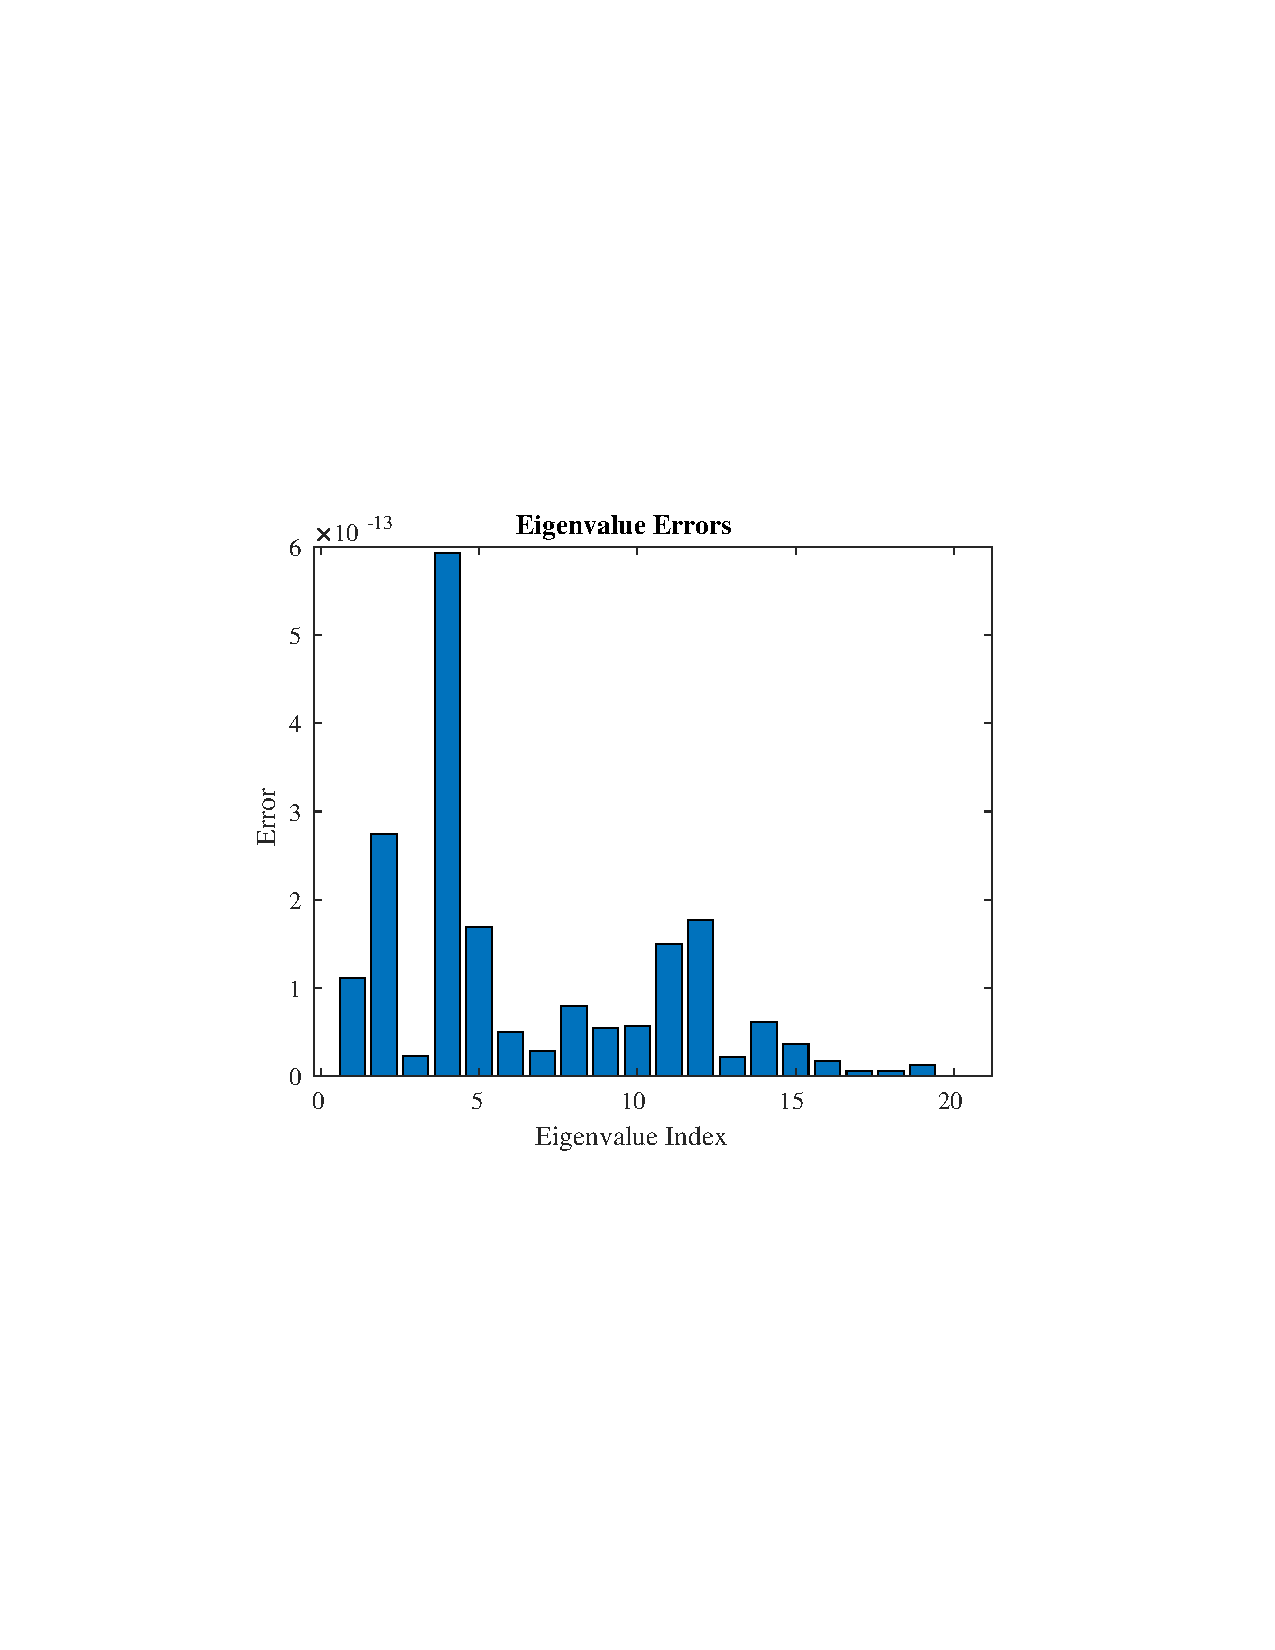
\includegraphics[width=\linewidth]{value_errors.pdf}
	\end{subfigure}
	~
	\begin{subfigure}[t]{0.49\linewidth}
		\centering
		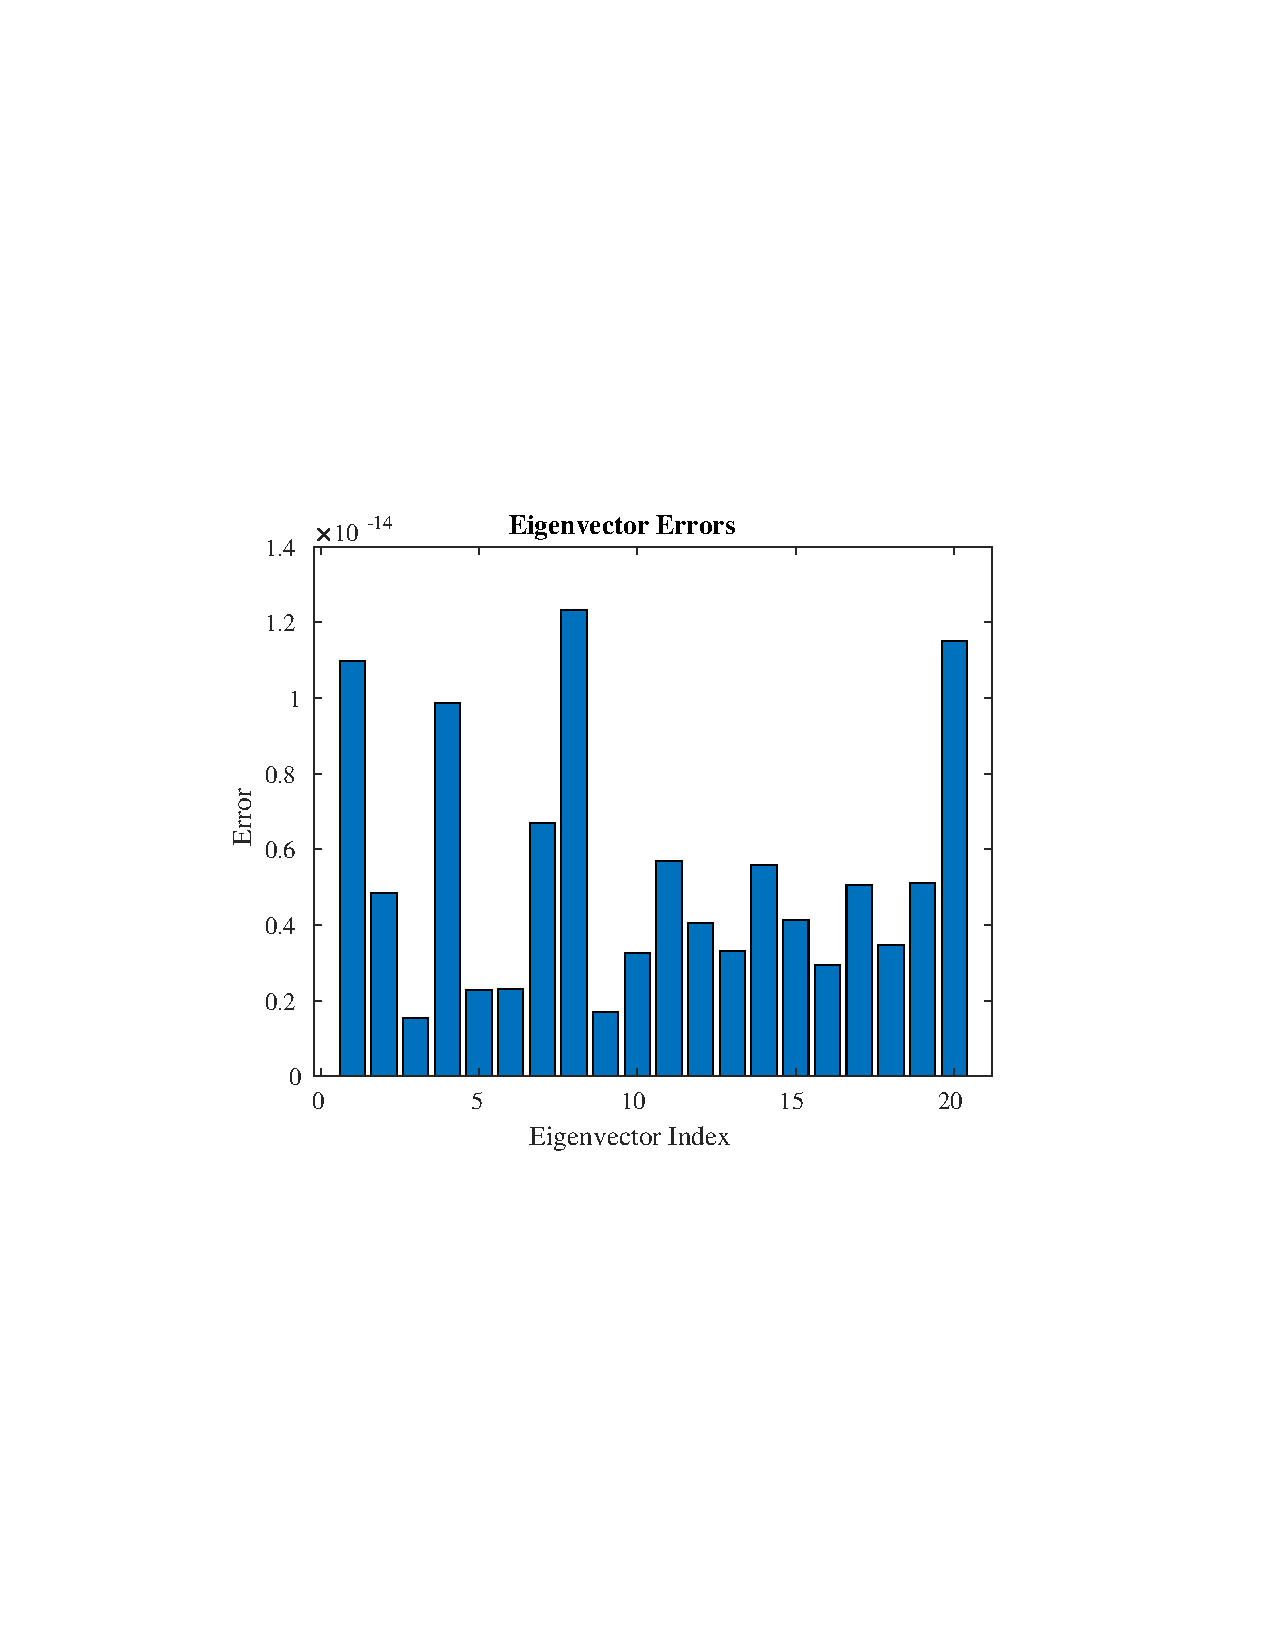
\includegraphics[width=\linewidth]{vector_errors.pdf}
	\end{subfigure}
	\caption{(Left) Absolute errors between the true eigenvalues and the eigenvalues computed using the QR method. (Right) $\ell^\infty$ errors between the true eigenvectors and the eigenvectors computed using the QR method.}
	\label{fig:errors1}
\end{figure}

Figure \ref{fig:errors1} shows the errors for the eigenvalues and eigenvectors using the basic QR method with stopping tolerance $\varepsilon = 10^{-12}$. We observe that all eigenvalues and eigenvector components are within roughly $10^{-12}$ of the true values, verifying that our implementation is correct. Furthermore, this validates the use of the stopping criterion in Algorithm \ref{alg:basic}.

\begin{figure}[htb!]
	\centering
	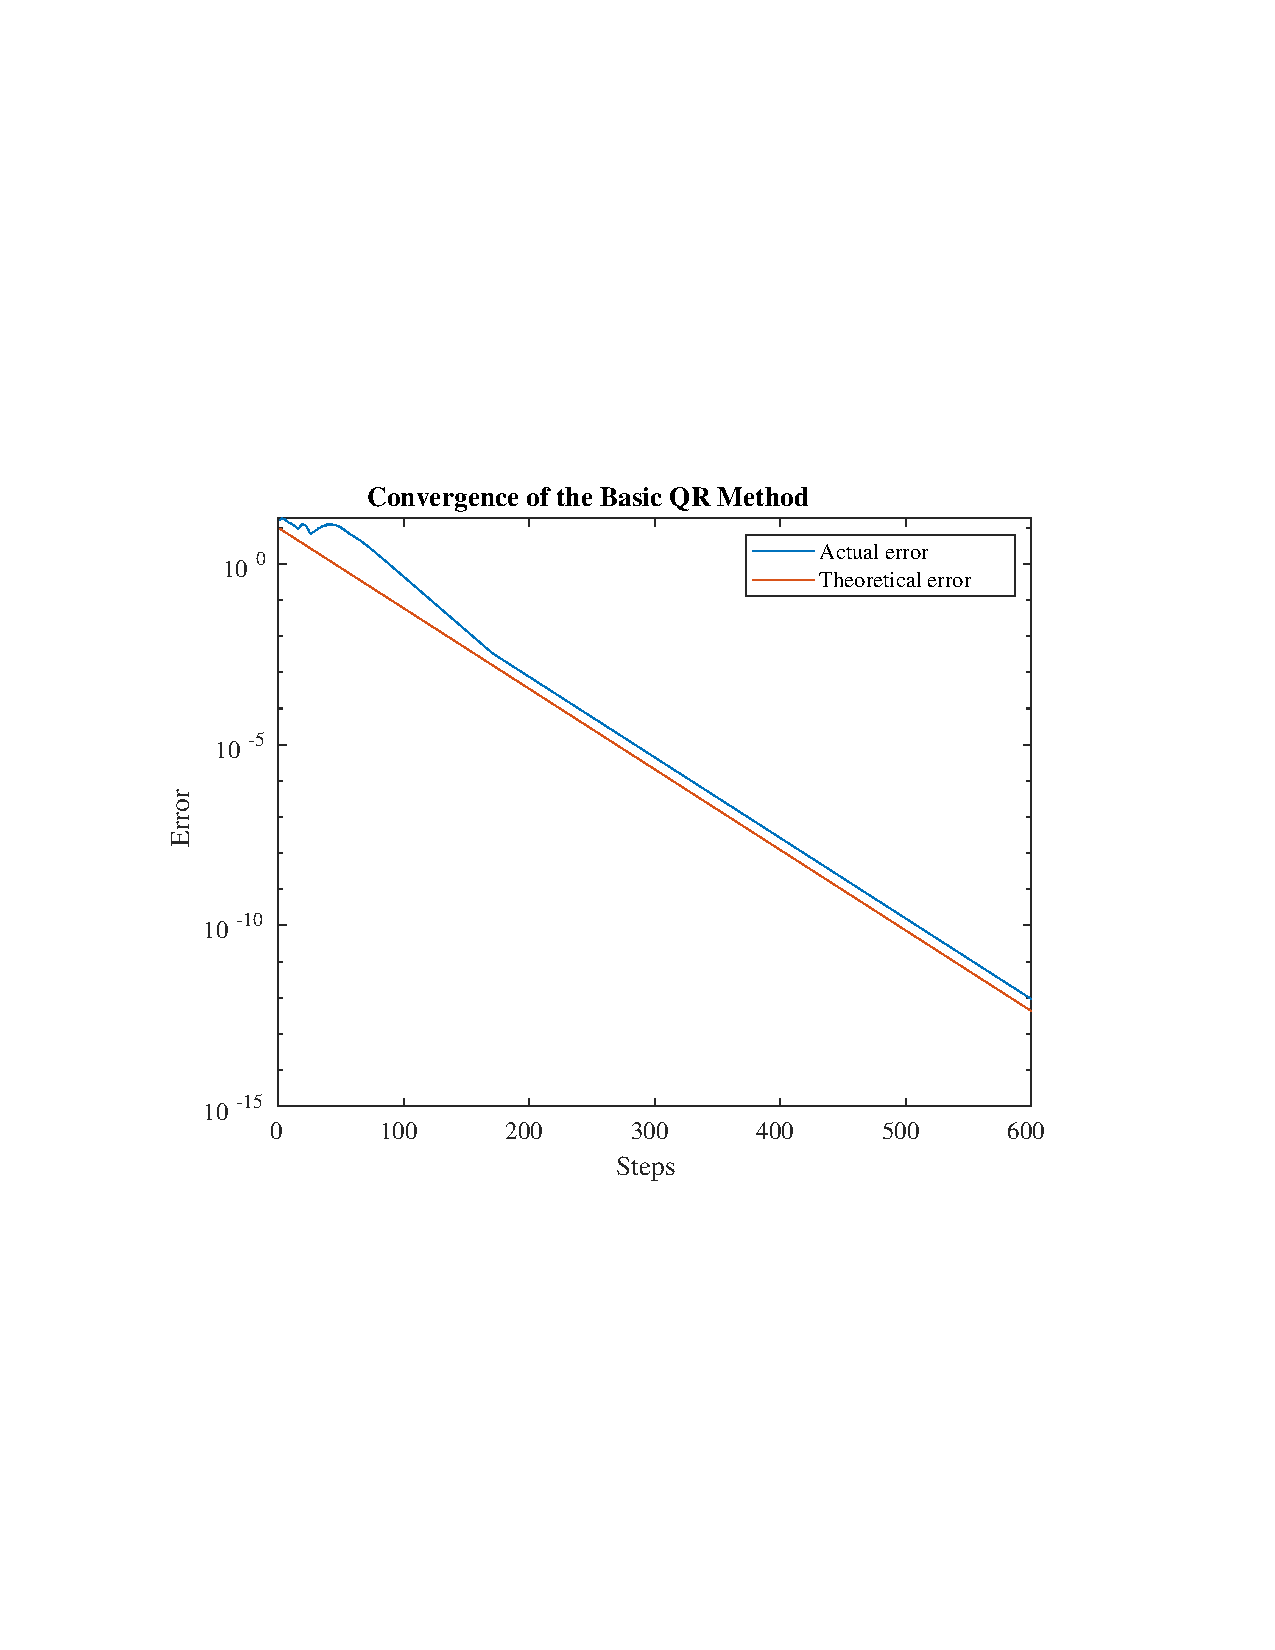
\includegraphics[width=0.7\linewidth]{convergence.pdf}
	\caption{Convergence of the basic QR method to an upper triangular matrix. The actual maximum absolute value of the lower triangular part of the iterates and the theoretical reference error $m(k)$ are plotted for each step $k$.}
	\label{fig:convergence}
\end{figure}

\subsubsection*{Part 2}
In this part we measure the stopping criterion for $A_k$, the maximum absolute value of the lower triangular entries of $A_k$, on each step $k$.
Figure \ref{fig:convergence} shows the maximum absolute value of the lower triangular entries of $A_k$. We observe that the error curve becomes parallel to the reference curve $m(k)$, which represents exponential decay in $k$. Since the plot uses a log scale on the error axis, this implies that the convergence of the basic QR method is $\bigoh(m(k))$, as predicted by Corollary \ref{cor:basic_convergence}.

\subsection{Convergence failures(?)}

In this section we demonstrate what happens when the QR method is applied to matrices that violate the assumptions of nonzero, separated eigenvalues. We implement this experiment in \texttt{experiment2.m}.

\subsubsection*{Part 1}
We start with a simple $3 \times 3$ matrix $A$ that has one real eigenvalue and two complex eigenvalues:
\begin{equation*}
	A = \mat{
		2 & 3 & 4 \\
		-2 & 1 & 0 \\
		1 & 2 & 0
	}.
\end{equation*}

We run 50 steps of the basic QR method on this matrix and obtain the following matrix $A_{50}$:
\begin{equation*}
	A_{50} \approx \mat{
		2.4093  &  -4.5482 &  -1.4324 \\
		1.4080  &  2.2739  &  0.6865 \\
		0  & 0  & -1.6832
	}.
\end{equation*}
We observe that $A_{50}$ is \emph{block upper triangular}. The value $-1.6832$ on the diagonal is very close to the real eigenvalue of $A$, and the eigenvalues of the upper-left $2\times 2$ submatrix of $A_{50}$ are very close to the complex eigenvalues of $A$.

Although the basic QR method is clearly not converging to an upper-triangular matrix, it does seem to be converging to a block upper triangular matrix, whose diagonal blocks can be used to find the eigenvalues of $A$. It is beyond the scope of this paper to prove it (even our textbook \cite{ackleh_2009} does not provide a proof, just the statement), but if $A$ is a real matrix, then the basic QR method always converges to a block upper triangular matrix\footnote{This is the reason for the ``?'' in section title. Although the QR method does not, in general, converge in the sense of Theorem \ref{thm:basic_method} specifically, it \emph{does} always converge in a more general sense.} whose diagonal blocks are either $1\times 1$, corresponding to real eigenvalues of $A$, or $2\times 2$, whose eigenvalues are complex eigenvalue pairs of $A$. The double QR method mentioned earlier is designed around exploiting this fact.

\subsubsection*{Part 2}
In this part we demonstrate the observations made in Part 1 on a larger scale. We generate a real, $10 \times 10$ matrix $B$ and run 1000 steps of the basic QR method on $B$. For one particular run, the output of which is stored in \texttt{experiment2\_output.txt}, we obtain the following matrix $B_{1000}$:
\begin{equation*}
	\small
	B_{1000} = \mat{
		{\color{red}5.0029}  & -0.4810  &  0.4937 &  -0.1995  &  0.3692  & -0.2716 &  -0.4672  &  0.2088  &  0.1050   & 0.1001 \\
		0 & {\color{red}-1.0326}  & -0.1319  & -0.1990 &   0.1406  & -0.1589  & -0.3451 &  -0.0119  & -0.1097  &  0.0197 \\
		0 & 0  & {\color{blue}-0.6263} &  {\color{blue}-0.3278}  &  0.0980  & -0.1330 &  -0.2053 &  -0.2685  &  0.1224  & -0.1714 \\
		0 & 0  &  {\color{blue}0.4937}  & {\color{blue}-0.7493} &   0.0624 &   0.5047  & -0.4036 &  -0.3831 &  -0.1645 &   0.1736 \\
		0 & 0 &  0  & 0 &  {\color{blue}-0.4732} &  {\color{blue}-0.8197}  &  0.4169  &  0.2311  &  0.2668 &   0.0755 \\
		0 & 0 & 0  &  0 &   {\color{blue}0.3931}  & {\color{blue}-0.2283}  & -0.2024  & -0.0914  & -0.2499  & -0.2570 \\
		0 & 0 &  0  &  0  &  0  &  0  &  {\color{blue}0.5741} &  {\color{blue}-0.1578} &  -0.2442  &  0.5990 \\
		0 & 0 &  0 &   0  &  0  &  0  &  {\color{blue}0.0874}  &  {\color{blue}0.5616} &   0.3131  & -0.0817 \\
		0 & 0 &  0  &  0  &  0  &  0  &  0  &  0  &  {\color{red}0.2517} &  -0.3398 \\
		0 & 0 &  0  &  0   & 0  &  0  &  0  &  0  &  0  & {\color{red}-0.1416}
	}.
\end{equation*}
Here we have indicated $1\times 1$ diagonal blocks in {\color{red}red} and $2\times 2$ diagonal blocks in {\color{blue}blue}. Checking the eigenvalues of these diagonal blocks against the true eigenvalues of $B$ verifies the observations in Part 1 (see \texttt{experiment2\_output.txt}).

\section{Conclusion}
In this project I learned about the QR method for finding all the eigenvalues and eigenvectors of a matrix $A$, which is an important problem, as eigenvalues and eigenvectors are useful in a wide range of applications. Indeed, the QR method is widely used in practical applications \cite{ackleh_2009}; however, I mostly studied the basic QR method, whose convergence is too slow to be useful in many cases. Additionally, the basic method only applies to matrices with separated eigenvalues. As mentioned, using origin shifts with deflation is the primary means by which the QR method is accelerated and applied to general matrices.

I derived the convergence rate of the basic QR method and conducted experiments demonstrating this convergence. I also demonstrated through my experiments why the assumption of separated eigenvalues is necessary for the QR method to converge; although, I also demonstrated that the convergence failure is not so bad, as QR method does still converge to \emph{something} when the eigenvalues of $A$ are not separated, and the eigenvalues and eigenvectors of $A$ can still be recovered from that \emph{something}. This shows how, with the proper modifications, the QR method can be one of the most general and powerful approaches to finding eigenvalues and eigenvectors numerically.


\clearpage
\bibliographystyle{mydefaultstyle.bst}
\bibliography{references}

\end{document}